% pdf/a 
\begin{filecontents*}[overwrite]{\jobname.xmpdata}
    \Title{}
    \Author{Gekkó csapat: Bak Bálint, Kozma Dávid Márk, Szilágyi Gábor}
    \Language{hu-HU}
    \Subject{Elektromágneses Terek házi feladat: Föld alatti fémkeresés örvényáramú vizsgálattal}
    \Keywords{EM szimuláció, végeselem, MATLAB, pdetool, házi feladat}
    \Publisher{Gekkó csapat}
\end{filecontents*}

\documentclass[a4paper,12pt,oneside]{article}
\usepackage{ucs}
\usepackage[T1]{fontenc}
\usepackage[utf8]{inputenc}
\usepackage[magyar]{babel}
\usepackage{amsfonts}
\usepackage{amsmath,bm}
\usepackage{pdfpages}
\usepackage{amssymb}
\usepackage{graphicx}
\usepackage[hang]{caption}
%\usepackage{subcaption}
%\usepackage{enumerate}
%\usepackage{psfrag}
\usepackage[left=10mm,right=10mm,top=10mm,bottom=10mm]{geometry}
\usepackage{hyperref}
%\usepackage{listings}
%\usepackage{cite}
%\usepackage{csquotes}
\usepackage[range-phrase=--, range-units=single]{siunitx}
\usepackage{xcolor}
\usepackage[a-3u]{pdfx}
\hypersetup{
    colorlinks,
%    linkcolor={red!50!black},
    linkcolor={black},
%    citecolor={blue!50!black},
    citecolor={black},
%    urlcolor={blue!80!black}
    urlcolor={blue!80!black}
}

\sloppy % Margón túllógó sorok tiltása.
\widowpenalty=10000 \clubpenalty=10000 %A fattyú- és árvasorok elkerülése
\def\hyph{-\penalty0\hskip0pt\relax} % Kötőjeles szavak elválasztásának engedélyezése

\pagestyle{plain} 
\pagenumbering{gobble}
\nopagebreak

\title{
    \centering
    \vspace{-0.8cm}
    
\includegraphics[width=0.3\textwidth]{bme_logo.pdf} \\
    \textbf{Elektromágneses Terek (VIHVMA08)\\
    csoportos házi feladat} \\[2ex]
    Föld alatti fémkeresés örvényáramú vizsgálattal
    \vspace{0.1cm}
}

%\parskip=10pt
%\parindent=0pt

\newcommand\adj[1]{#1^{\mathrm{H}}}

\author{\emph{\textbf{Gekkó}} csapat:~Bak Bálint,~Kozma Dávid Márk,~Szilágyi Gábor \\[2ex]
    Konzulens: Dr. Pávó József}
\date{Budapest, \today}


\begin{document}
    \maketitle
%   
    \section{Bevezetés}
    A feladatkiírásban felvázolt probléma egy forgásszimmetrikus elrendezés, emiatt \aref{fig:elrendezes_2d}. ábrán látható fél-síkmetszet vizsgálata elég a probléma megoldásához.

    \begin{wrapfigure}{L}{0.35\textwidth}
        \centering
        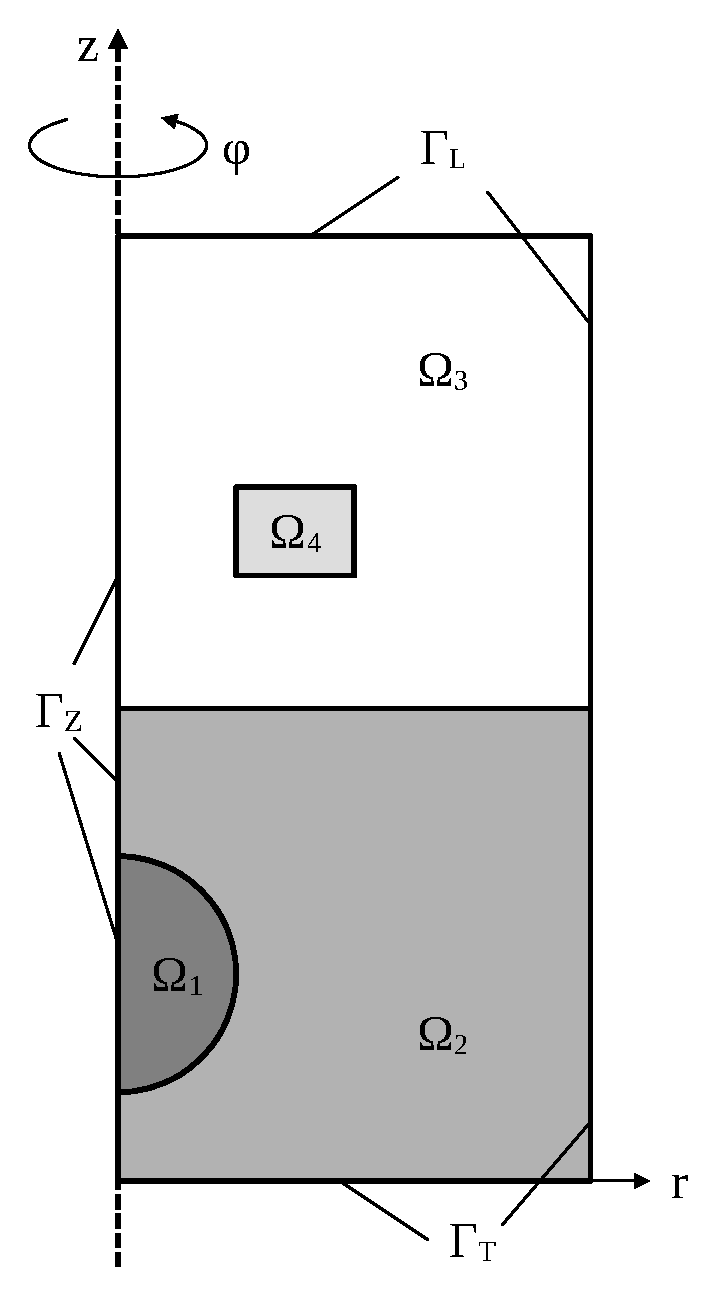
\includegraphics[width=0.9\linewidth]{elrendezes_2d.pdf}
        \caption{A szimulált elrendezés.}
        \label{fig:elrendezes_2d}
    \end{wrapfigure}

    \begin{align}
        \dfrac{\partial}{\partial \varphi} = 0
    \end{align}
    
    A tartományok jelentése: $\Omega_1$ -- vasgömb, $\Omega_2$ -- talaj, $\Omega_3$ -- levegő, $\Omega_4$ -- tekercs.

    Mivel csak egy adott $\omega$ körfrekvencián kell vizsgálódnunk, emiatt elég a szinuszos állandósult állapottal foglalkoznunk:
    \begin{align}
        \dfrac{\partial}{\partial t} \quad&\longrightarrow\quad j\omega
    \end{align}
    A kérdéses $\omega$ körfrekvencián az elektromágneses hullámok szabadtéri hullámhossza ($\varepsilon_r = 1$):
    \begin{align}
        \lambda &= \dfrac{c}{f} = \dfrac{c}{\dfrac{\omega}{2\pi}} = \dfrac{\qty{3e8}{\metre\per\second}}{\dfrac{2\pi\qty{500}{\per\second}}{2\pi}} = \qty{6e5}{\metre}
    \end{align}
    Emiatt $\lambda$ az \qty{1000}{km} nagyságrendjébe esik, míg az elrendezés fizikai méretei néhányszor \qty{10}{cm}-esek, így élhetünk a magneto-kvázistacionárius közelítéssel:
    \begin{align}
        \dfrac{\partial \vec{D}}{\partial t} \quad&\longrightarrow\quad 0
    \end{align}
    \clearpage
    Ebben az esetben a vizsgált tartományon belül a Maxwell-egyenleteknek a következő alakja érvényes:
    \begin{align}
        \rot \vec{H} &= \vec{J} \\
        \rot \vec{E} &= -j\omega\vec{B}\\
        \divergence \vec{B} &= 0\\
        \vec{B} &= \mu\vec{H}\\
        \vec{J} &= \sigma \vec{E} + \vec{J}_i
    \end{align}

    \begin{align}
        \sigma(\vec{r}) &=
            \begin{cases}
                \sigma, & \text{ha } \vec{r} \in \Omega_1\\
                \sigma_t, & \text{ha } \vec{r} \in \Omega_2\\
                0, & \text{ha } \vec{r} \in \Omega_3 \cup \Omega_4
            \end{cases}
    \end{align}

    Az $R$ sugarat megfelelően nagyra kell választani ahhoz, hogy a kialakuló teret ne befolyásolja jelentősen a vizsgált $\Omega$ tartomány $\Gamma_T \cup \Gamma_L$ ,,távoli'' peremének a közelsége.
    

    \section{Bak Bálint szekciója}
    dolgok

    \section{Kozma Dávid Márk szekciója}
    dolgok

    A feladat megoldásához az $\vec{A}-\Phi, \vec{A}$ formalizmust használjuk, mert az előadáson bemutatott indukciós főzőlapos példa alapján ezzel a megközelítéssel egy jól kezelhető parciális differenciálegyenlet-rendszert kapunk, amit a PDEtool segítségével megoldhatunk.
\begin{align}
    \vec{B} = \rot \vec{A}
\end{align}
A peremfeltételekről a következőket lehet tudni:
\begin{align}
    B_n(\vec{r}) &= 0, \quad \vec{r} \in \Gamma_Z\\
    B_n(\vec{r}) &= 0, \quad \vec{r} \in \Gamma_L \cup \Gamma_T
\end{align}
A $B_n$ normális mágneses indukció a $\Gamma_Z$ peremen a szimmetria miatt lesz 0, a $\Gamma_L \cup \Gamma_T$ távoli peremeken pedig a nagy távolság miatt lesz közel 0, amit pontosan 0 értékkel modellezünk.
\section{A PDE és megadása pdetool-ban}
A tartományokra vonatkozó parciális differenciálegyenlet:
\begin{equation}
    -\left(\dfrac{\partial}{\partial r}\dfrac{1}{r\mu}\dfrac{\partial(rA_{\varphi})}{\partial r}+\dfrac{\partial}{\partial z}\dfrac{1}{r\mu}\dfrac{\partial(rA_{\varphi})}{\partial z}\right) + j\omega\sigma A_{\varphi} = J_{i,\varphi}
\end{equation}
Ezt a következő helyettesítésekkel lehet MATLAB-ban (pdetool-ban) megadni:
\begin{equation}
    \begin{aligned}
        rA_{\varphi}\quad\rightarrow&\quad\verb|u|\\
        r\quad\rightarrow&\quad\verb|x|\\
        z\quad\rightarrow&\quad\verb|y|
    \end{aligned}
\end{equation}
A használt elliptikus PDE séma a következő:
\begin{equation}
    \verb|-div(c*grad(u))+a*u=f|
\end{equation}
Eszerint az egyes paraméterek behelyettesítési értékei:
\begin{equation}
    \begin{aligned}
        \verb|c|\quad=&\quad\dfrac{1}{r\mu}\\
        \verb|a|\quad=&\quad\dfrac{j\omega\sigma}{r}\\
        \verb|f|\quad=&\quad J_{i,\varphi}
    \end{aligned}
\end{equation}

    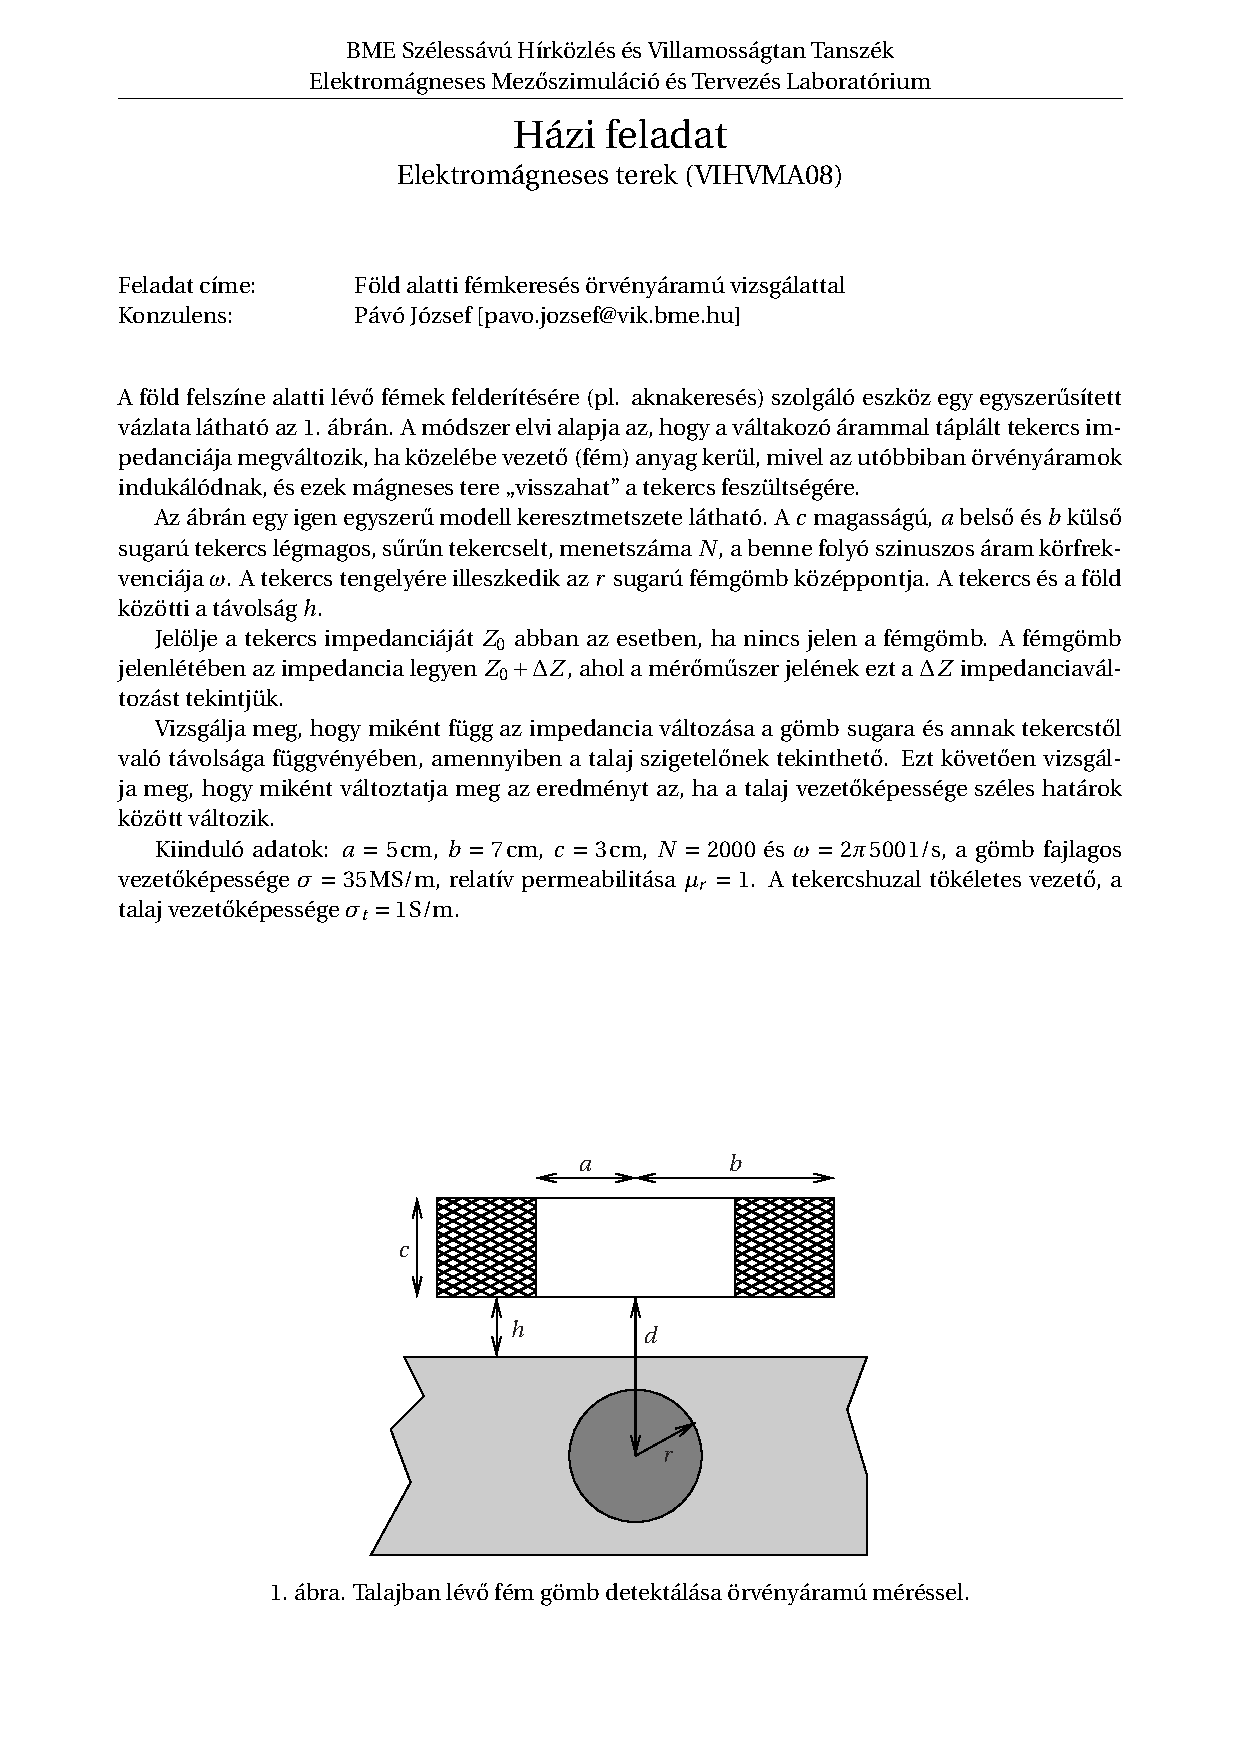
\includepdf{feladatlap_femkereses.pdf}
%
\end{document}

%            \begin{figure}
%                \centering
%                \includegraphics[width=0.8\textwidth]{kep/szerkesztett/wstk-mighty-gecko-nagy.jpg}
%                \caption{WSTK + radio board.}
%                \label{fig:wstkmighty}
%            \end{figure}
% \cite{Anritsu}
%            \begin{figure}
%                \centering
%                \begin{subfigure}{0.48\textwidth}
%                    \includegraphics[width=\textwidth]{kep/szerkesztett/sol-868-conducted.png}
%                    \caption{\SI{868}{MHz}}
%                \end{subfigure}
%                \begin{subfigure}{0.48\textwidth}
%                    \includegraphics[width=\textwidth]{kep/szerkesztett/sol-470-conducted.png}
%                    \caption{\SI{470}{MHz}}
%                \end{subfigure}
%                \caption{470 és \SI{868}{MHz}-es Sol radio board-ok kimeneti spektruma.}
%                \label{fig:sol-conducted}
%            \end{figure}

